% Chapter 5

\chapter{Produzione} % Main chapter title

\label{Chapter5} % Change X to a consecutive number; for referencing this chapter elsewhere, use \ref{ChapterX}

%----------------------------------------------------------------------------------------
%	SECTION 1
%----------------------------------------------------------------------------------------

\section{Modellazione}

Con modellazione digitale, o modellazione 3D, o semplicemente modellazione, per brevità, si intende la manipolazione di veritci in uno spazio tridimensionale per realizzare solidi più o meno complessi denominati modelli.
Questa è senz'altro la fare più artistica dell'intero processo di produzione, e una di quelle che più mi ha appassionato.

Una volta definiti i concept art, in gran parte realizzati da A. Uras, il primo passo della produzione è appunto quello di realizzare i modelli dei personaggi, dei prop e delle ambientazioni.
Per fare ciò, sono state usate diverse tecniche di modellazione 3D, che possono essere divise nelle seguenti due categorie:
\begin{itemize}
    \item Modellazione hard-surface \cite{hardSurf}.
    \item Scultura digitale\cite{3Dsculpt}.
\end{itemize}
La differenza fondamentale sta nel cosa si vuole realizzare. La prima è ottima per quasi tutto ciò che è realizzato dall'uomo (e.g. macchinari, edifici) ed è stata quindi stata usata nella realizzazione di ambientazioni e prop.
Consiste nel partire da una forma geometrica semplice, ad esempio un cubo o una sfera, ed aggiungere dettagli estrudendo sezioni o utilizzato operatori booleani in combinazione con altre forme geometriche. (Figura \ref{fig:box-model})
Il risultato è un modello dagli spigoli ben definiti, che comunque può avere superfici curve e smussate.
La caratteristica che lo distingue è la simmetria della struttura e la precisione della posizione dei dettagli. 

\begin{figure}
\centering
\begin{subfigure}{.5\textwidth}
  \centering
  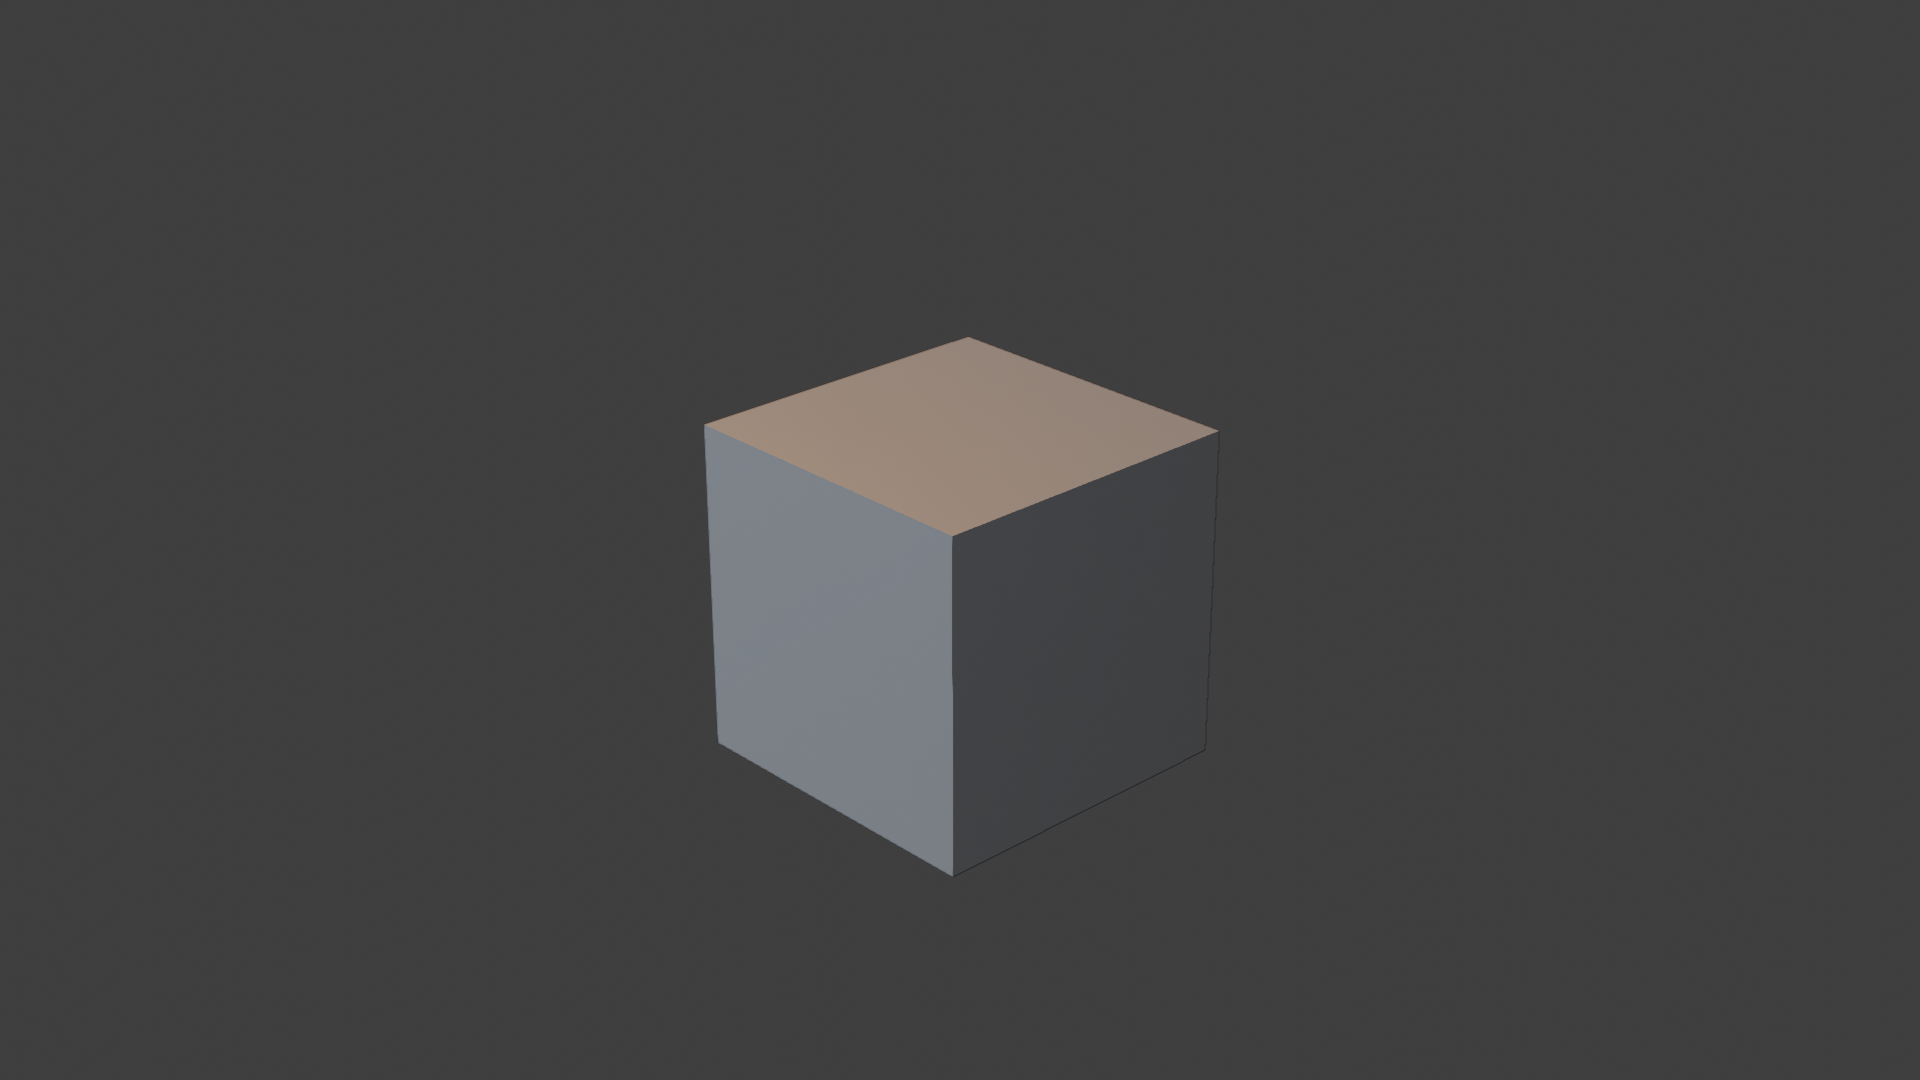
\includegraphics[width=.99\linewidth]{Figures/box1.png}
\end{subfigure}%
\begin{subfigure}{.5\textwidth}
  \centering
  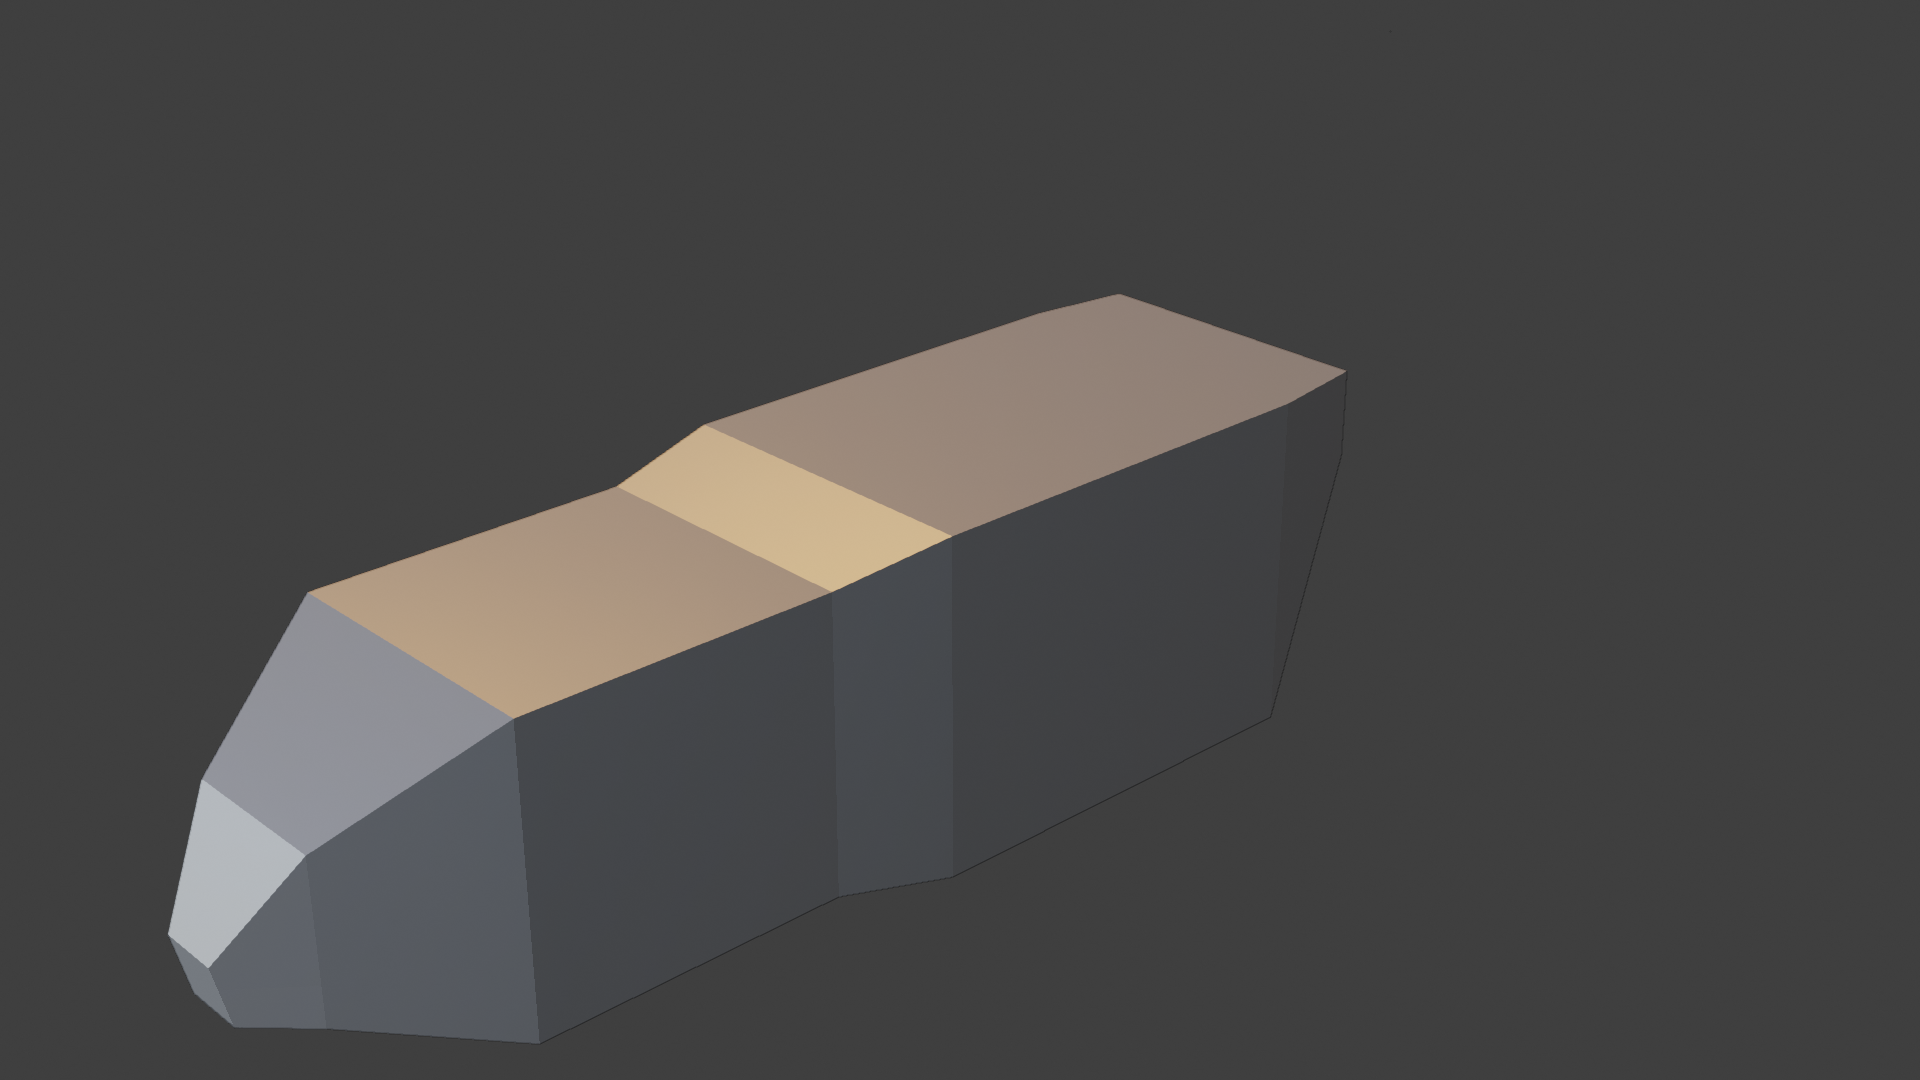
\includegraphics[width=.99\linewidth]{Figures/box2.png}
\end{subfigure}
\begin{subfigure}{.5\textwidth}
  \centering
  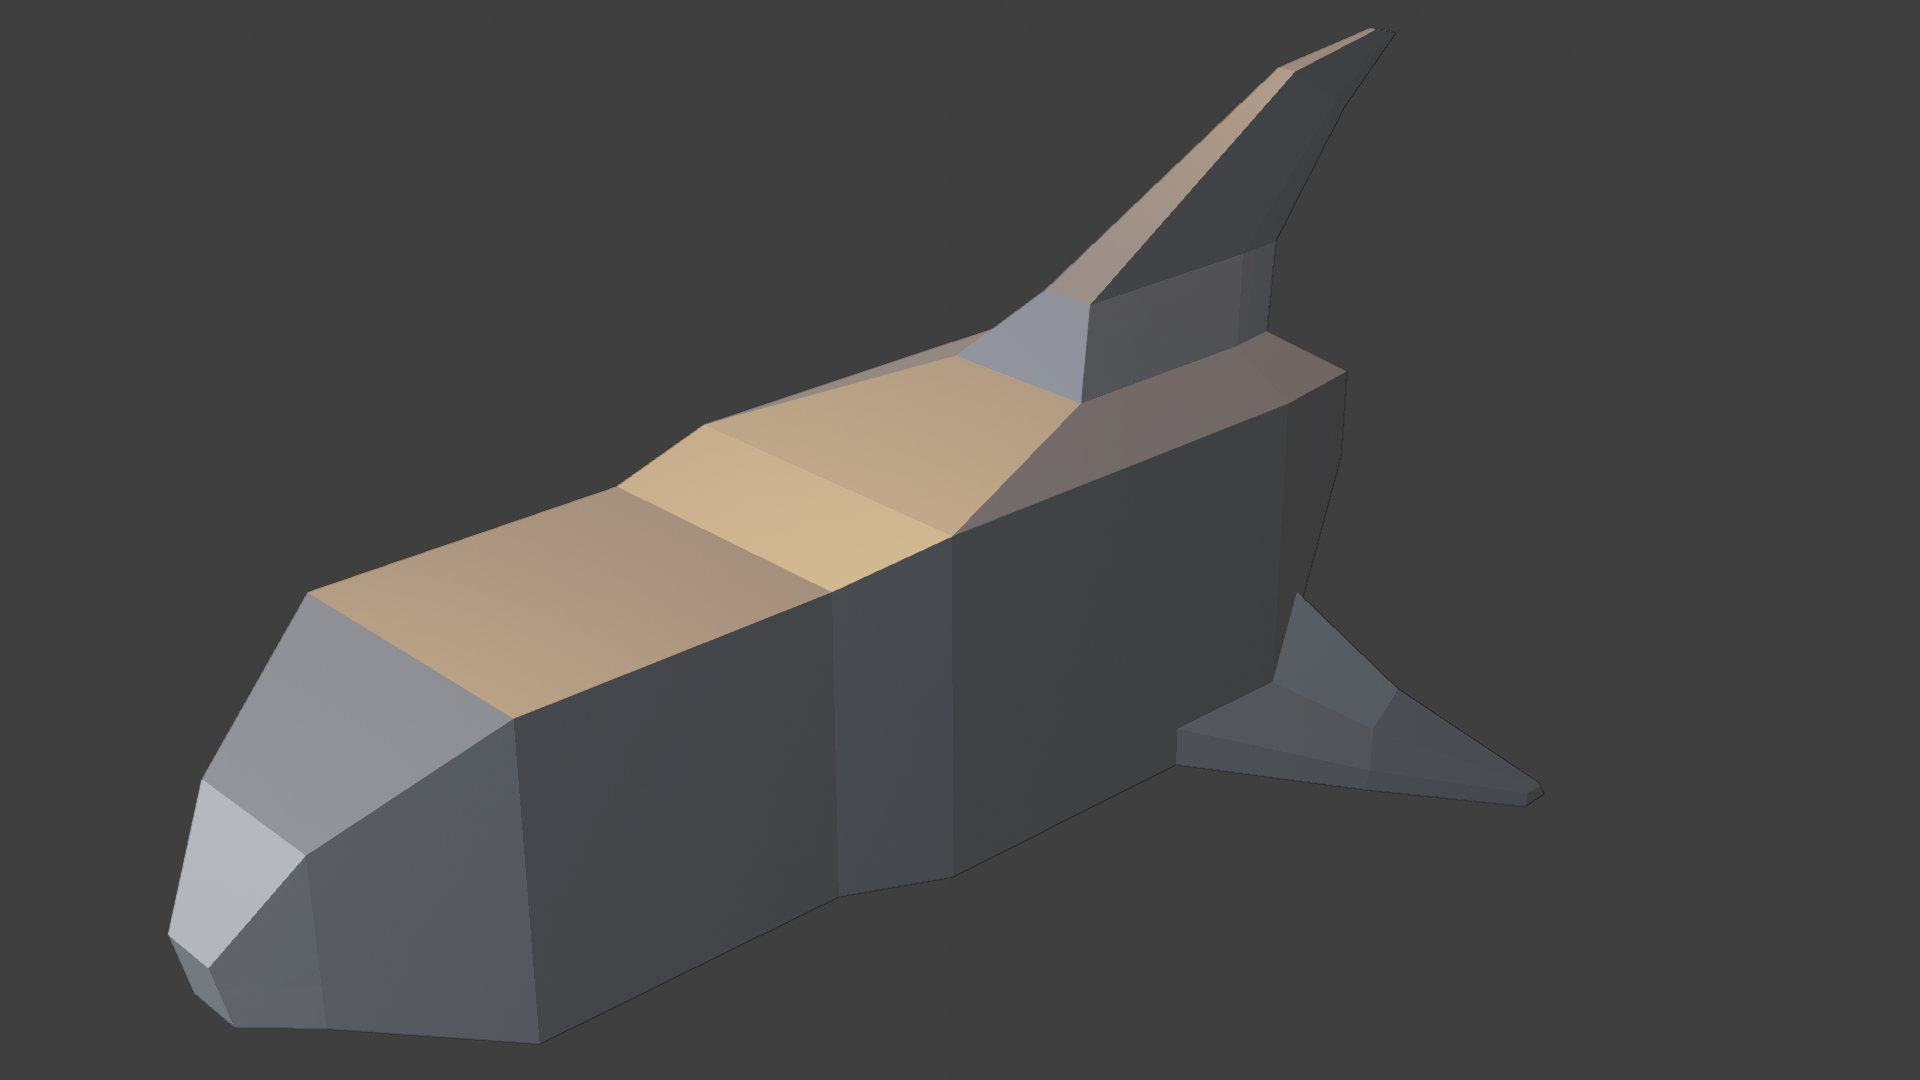
\includegraphics[width=.99\linewidth]{Figures/box3.png}
\end{subfigure}%
\begin{subfigure}{.5\textwidth}
  \centering
  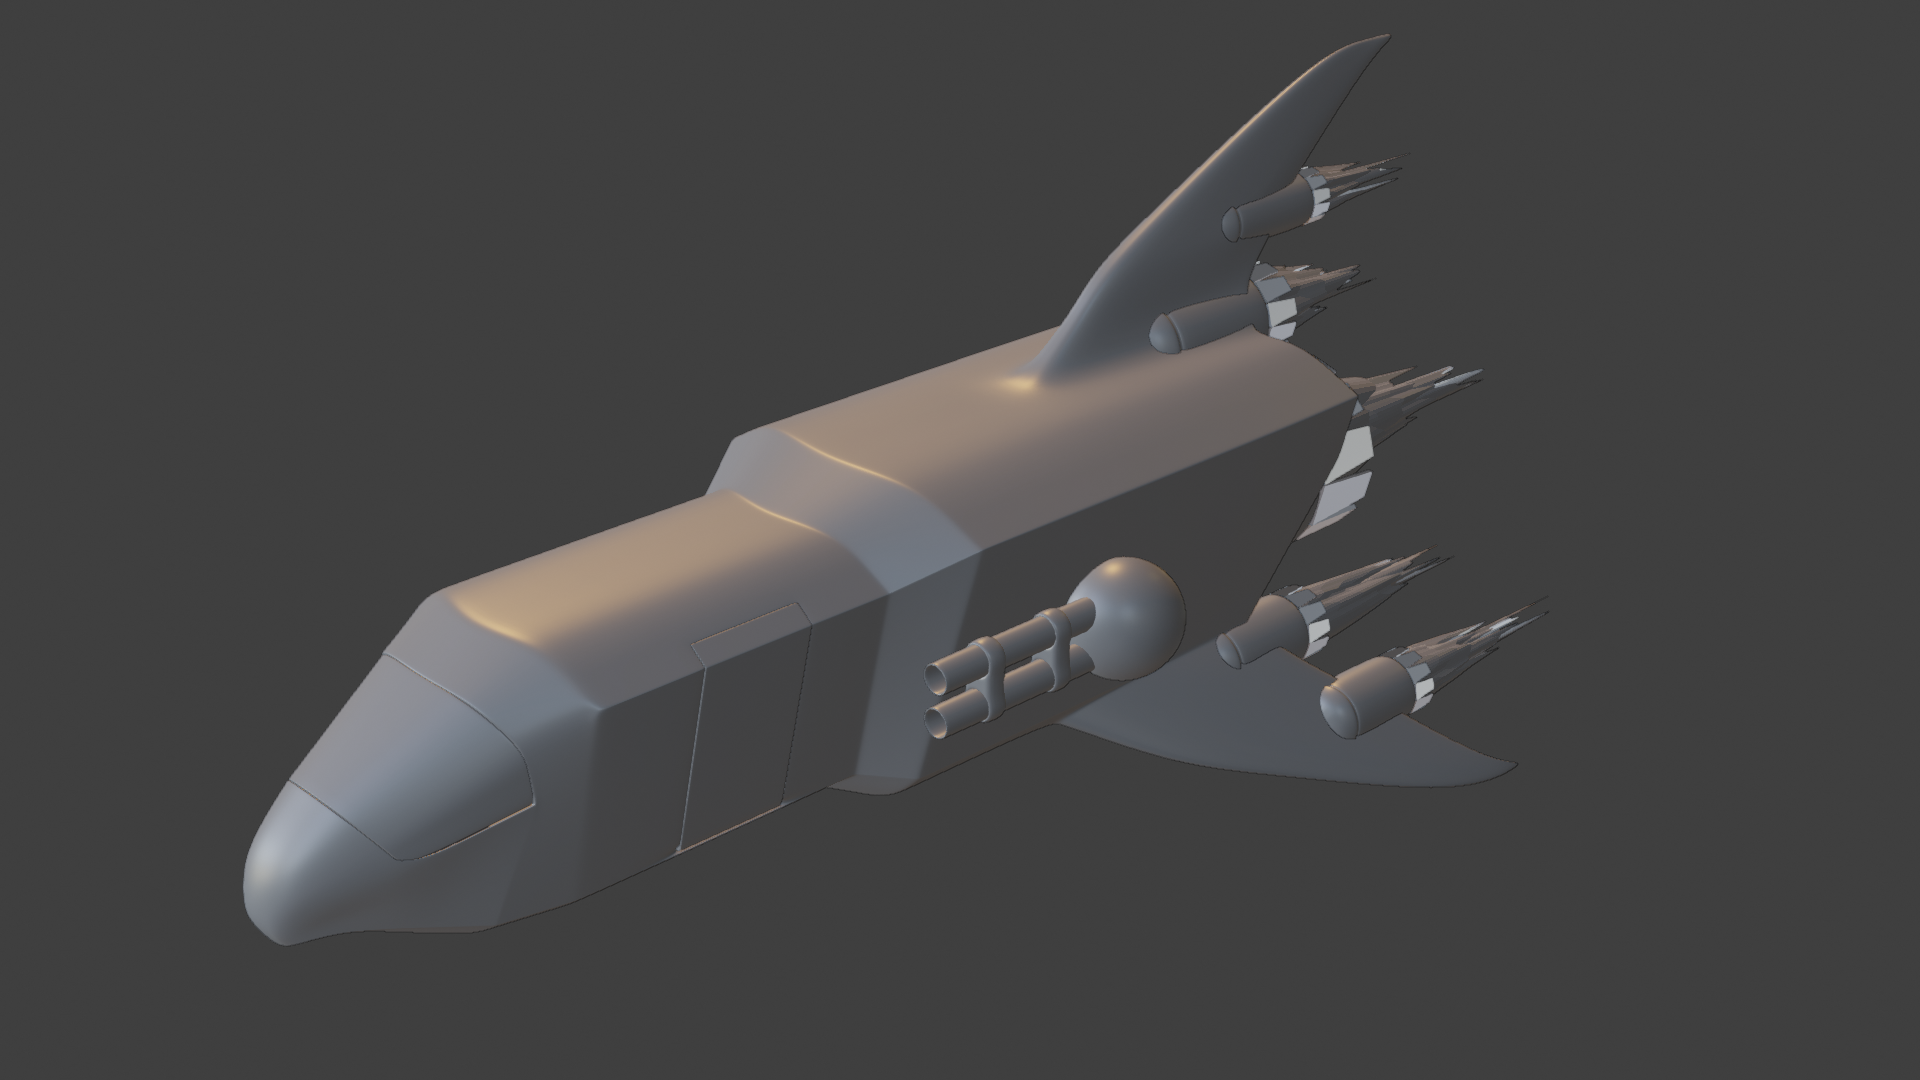
\includegraphics[width=.99\linewidth]{Figures/box4.png}
\end{subfigure}\\[2ex]
\decoRule
\caption[Modellazione hard-surface]{Esempio di modellazione hard-surface per modellare un'astronave.}
\label{fig:box-model}
\end{figure}

Al contrario, il secondo metodo viene utilizzato per ottenere modelli organici, in pratica tutto ciò che è presente in natura.
Questi modelli sono particolari, poiché andranno deformati per essere animati.
Un esempio lampante, in questo progetto, sono i personaggi.
Nonostante anche in questo caso la simmetria sia fondamentale (ogni personaggio ha due braccia e due gambe perfettamente simmetriche), vengono solitamente aggiunti dettagli per rompere la simmetria, siccome in natura nulla è perfettamente simmetrico.
Anche in questo caso si parte solitamente da forme geometriche semplici, tuttavia il processo di modellazione è completamente differente, tant'è che spesso si fa distinzione tra modellazione e scultura digitale (come se i due concetti si escludessero a vicenda).
Nella scultura digitale infatti non si usano mai operazioni come l'estrusione di una faccia, di fatto il concetto di faccia non viene neanche utilizzato.
La mesh viene vista come un oggetto compatto, i cui vertici possono essere manipolati attraverso strumenti che emulano le azioni di uno scultore.
Per questo motivo la scultura digitale è anche il metodo di modellazione preferito dagli artisti.
\newline

\begin{figure}
\centering
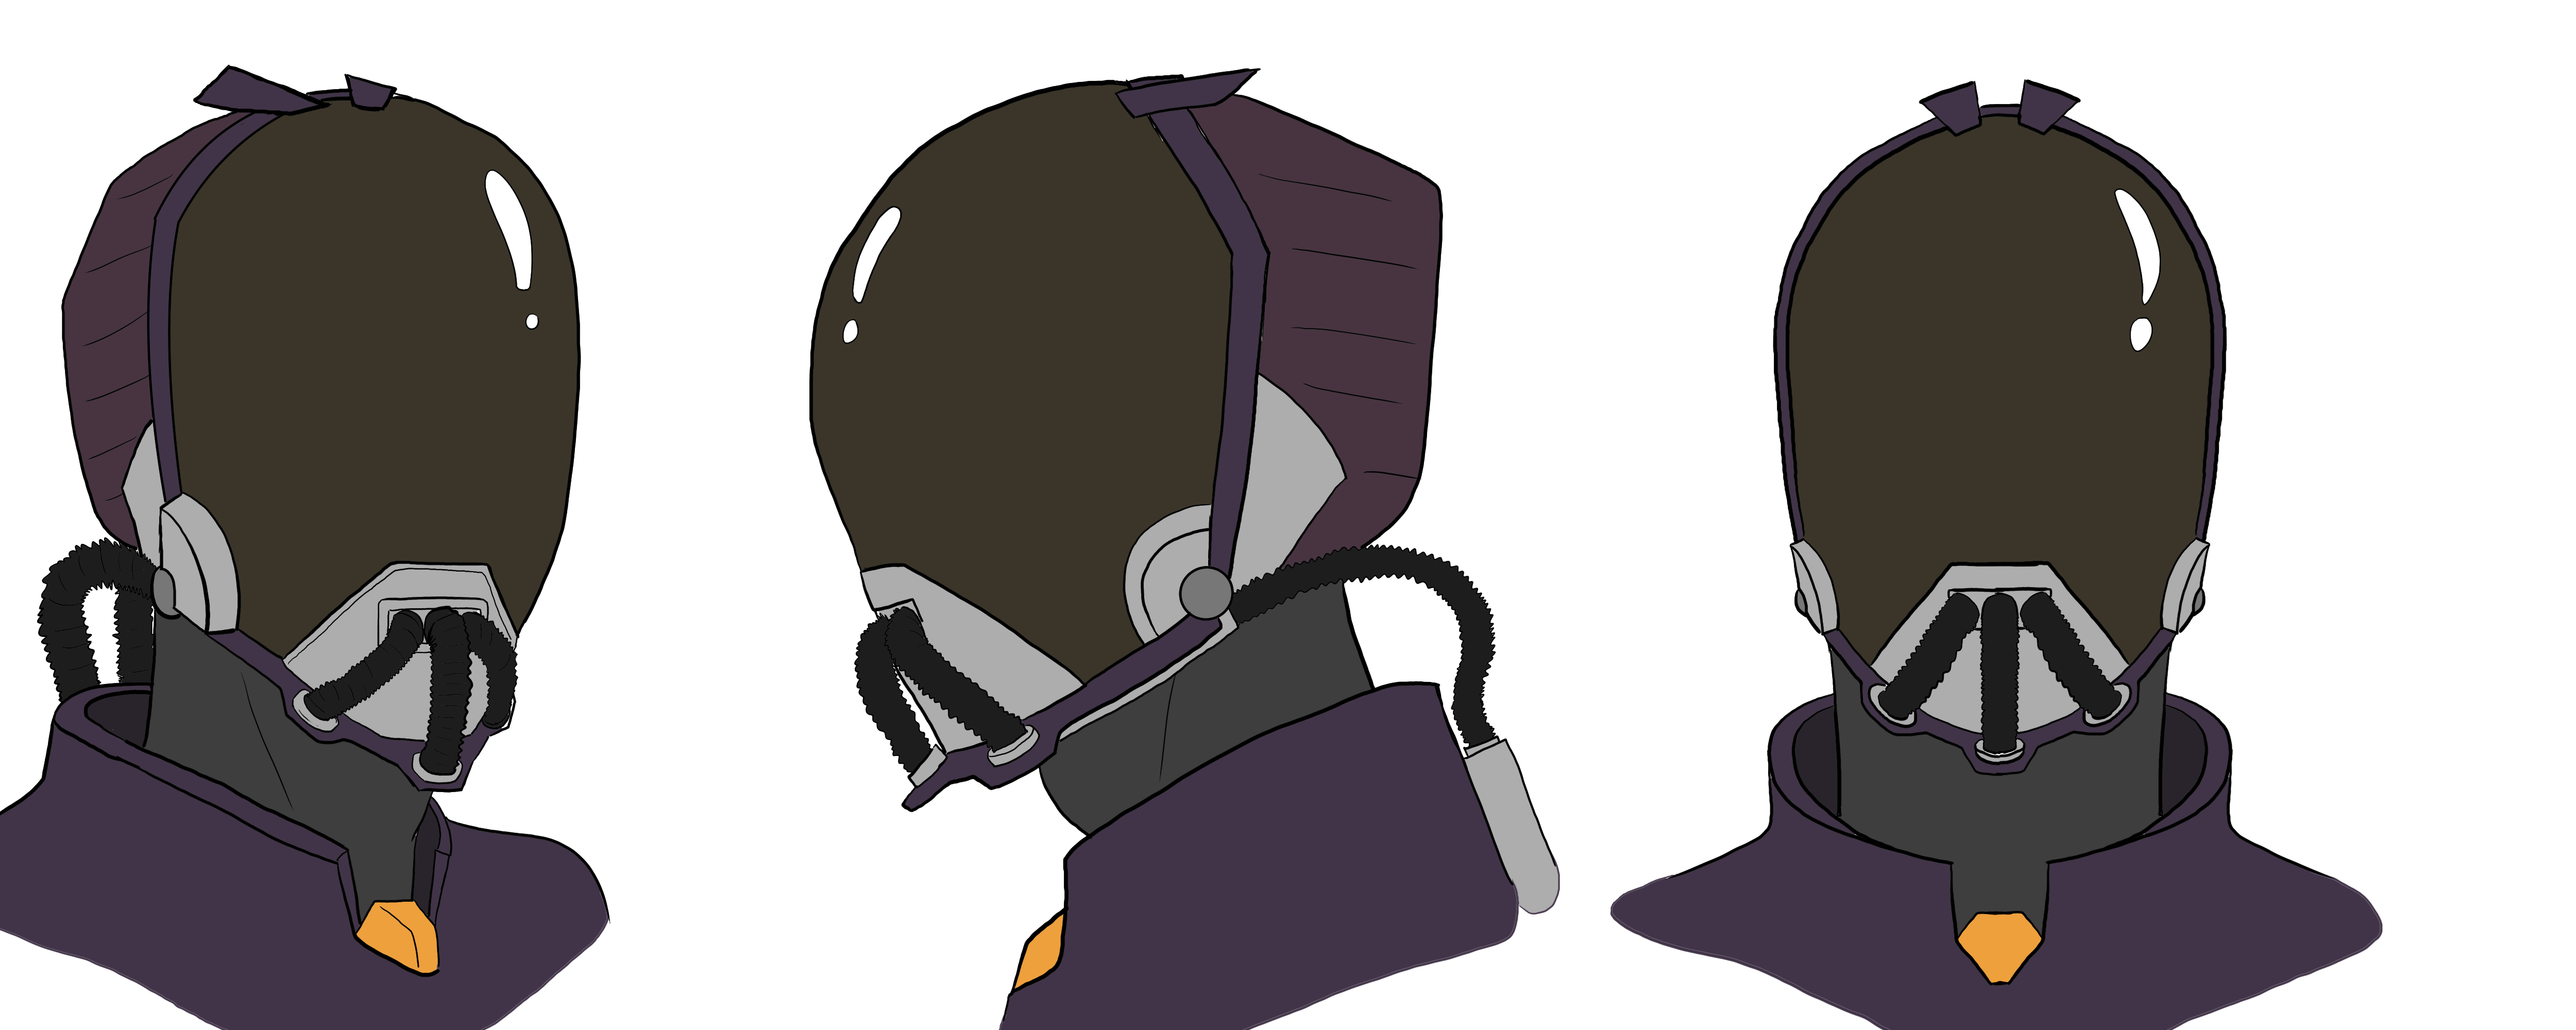
\includegraphics[width=.8\textwidth]{Figures/bandit-concept}
\decoRule
\caption[Concept art]{Concept art di uno dei porsonaggi}
\label{fig:concept}
\end{figure}
\begin{figure}
\centering
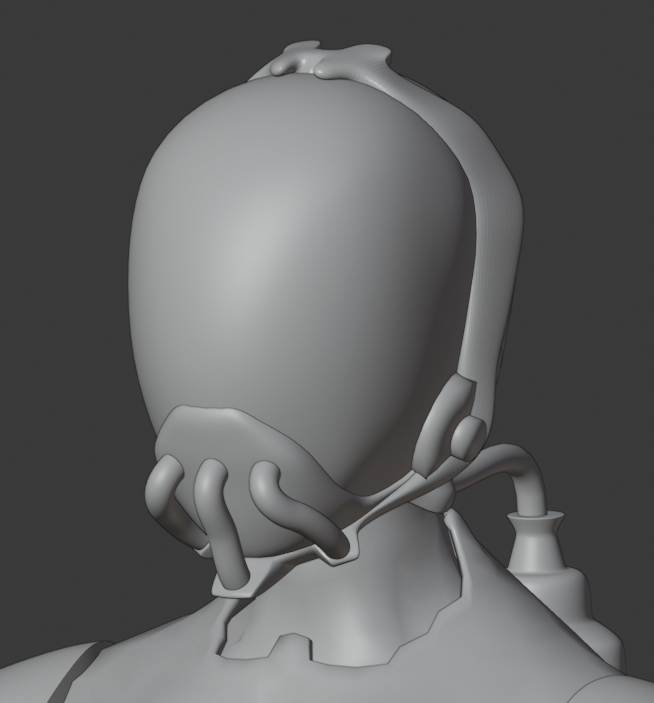
\includegraphics[width=.8\textwidth]{Figures/bandit-head}
\decoRule
\caption[Modello 3D]{Rappresentazione 3D del concept art mostrato in Figura \ref{fig:concept}}
\label{fig:model}
\end{figure}
Affinché un modello si possa definire ben fatto e ultimato, è necessario soddisfare i seguenti criteri.
In primo luogo, deve ben rappresentare in 3D quello che il concept si limitava a mostrare in 2D.
In Figura \ref{fig:concept} e \ref{fig:model} è possibile notare quanto il modello 3D si avvicini al concept originale.
Nonostante, in questo caso, il modello rappresenti molto bene il concept, è possibile notare come alcuni dettagli differiscano.
Questo è dovuto principalmente a due motivi: il primo è che, semplicemente, il concept art serve a dare un'idea di come deve apparire il personaggio, e non vincola quindi a mantenere gli stessi dettagli durante la fase di modellazione.
Il secondo è che in un disegno 2D la forzatura della prospettiva può nascondere dettagli a cui un modello 3D non può evadere.
Per tanto, sono spesso necessarie modifiche poiché non sarebbe possibile realizzare in 3D ciò che era rappresentato in 2D.

\begin{figure}
\centering
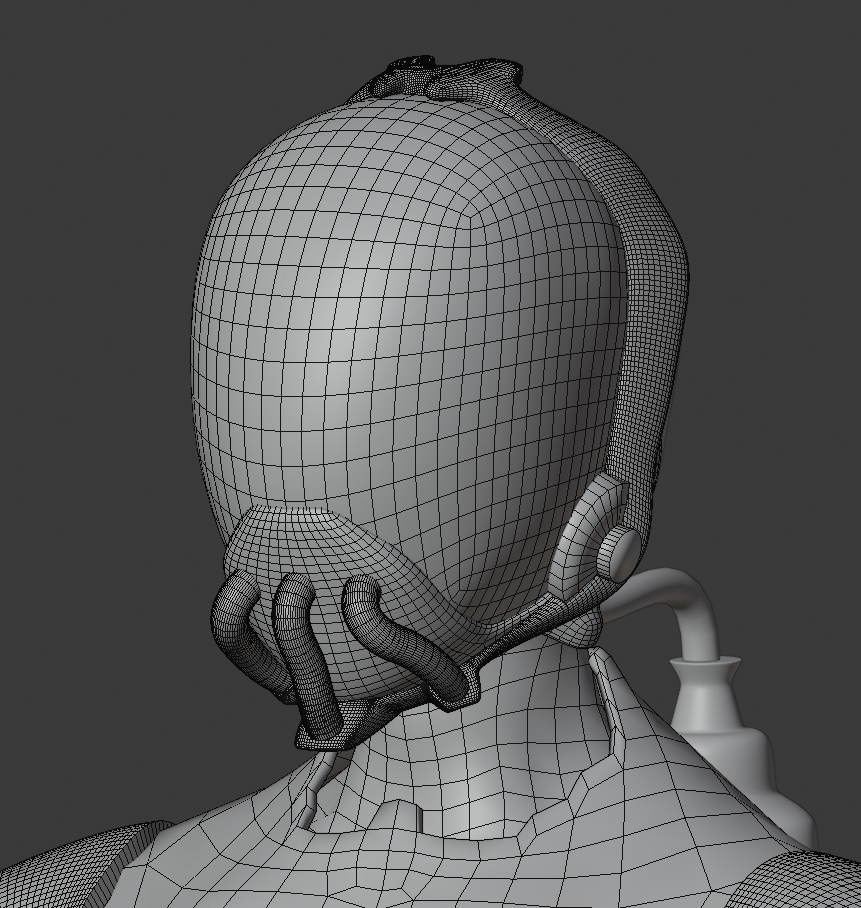
\includegraphics[width=.8\textwidth]{Figures/bandit-wire}
\decoRule
\caption[Topologia]{Modello 3D con topologia della mesh visibile}
\label{fig:wire}
\end{figure}
Il secondo criterio, non meno importante del primo, è la \emph{topologia} della mesh.
A dir la verità, questo aspetto non ha alcuna importanza nel caso di modelli statici, mirati allo scopo di essere rappresentati in un render fisso, o stampati in 3D.
Tuttavia, nel caso delle animazioni, questo è un aspetto fondamentale.
Infatti dal posizionamento dei vertici dipende la deformazione della mesh che, com'è già stato detto, è necessaria nelle animazioni dei modelli organici (e.g. personaggi).
Per avere una buona topologia, è fondamentale che le facce siano composte di quattro lati. Questo serve a definire dei percorsi, che attraversano la faccia da un lato a quello opposto e continuano nelle facce adiacenti.
Questi percorsi servono a far si che quando si aggiunge un maggiore livello di dettaglio, la mesh non venga deformata in maniera inaspettata.
Un altra caratteristica importante, per una buona topologia, è quella di avere al massimo quattro spigoli (o archi) che partano da ogni vertice.
Questo non è sempre possibile, tuttavia è necessario che vertici con più di cinque spigoli siano presenti nel minor numero possibile, e siano posizionati in punti strategici dove la mesh verrà difficilmente deformata.
Questo perché se vertice è adiacente a molti vertici, genera anche molti incroci di percorsi che sono da evitare per quanto detto prima.

Infine, un aspetto non poco importante nella definizione qualitativa di un modello, è il numero totale di vertici.
L'obiettivo è quello di avere il minor numero possibile di vertici per poter realizzare un certo livello di dettaglio.
Il motivo anche qui è duplice, seppure i due effetti sono strettamente correlati.
Innanzi tutto, un ridotto numero di vertici permette un \emph{frame-rate} più alto in fase di animazione.
In secondo luogo, in fase di rendering, ogni frame impiegerà meno tempo ad essere renderizzato.

Per mantenere un livello di dettaglio, discretamente alto, è stato fatto uso di una tecnica denominata \emph{baking}, che verrà approfondita nel paragrafo successivo.
Per ora mi limiterò a dire che per ogni modello è stato fatta prima una versione "\emph{low-poly}", ovvero a basso contenuto di poligoni (o vertici, analogamente).
Dopodiché i dettagli sono stati modellati su una copia di questo modello, dopo averne aumentato il numero di vertici suddividendo ogni faccia.
Avere due modelli separati, ci permette di utilizzare il primo nelle animazioni e, in un secondo momento, aggiungere i dettagli "cucinati".

Qui i vantaggi sono molteplici: è possibile iniziare ad animare un modello subito, parallelizzando la fase di animazione a quella di modellazione dei dettagli.
In più come già detto, si avrà un frame-rate più alto in fase di animazione, ed un rendering più veloce una volta ultimate le animazioni.

In Figura \ref{fig:boy} \ref{fig:cap} \ref{fig:lt} e \ref{fig:prop} sono riportati altri esempi di comparazione tra concept e modello 3D dei modelli da me realizzati. Tutti i concept, a parte quello del tenente, sono stati forniti da Alberto Uras. 
\begin{figure}
\centering
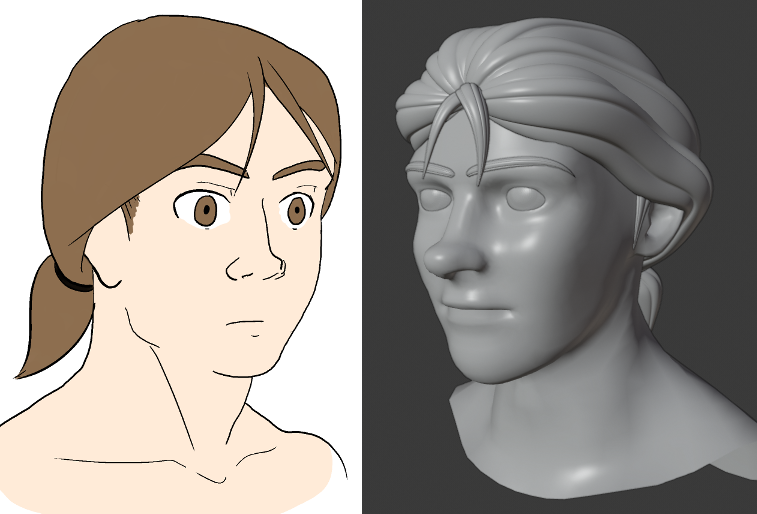
\includegraphics[width=.8\textwidth]{Figures/boy}
\decoRule
\caption[Ragazzo]{Modello 3D del volto del ragazzo a confronto con il relativo concept.}
\label{fig:boy}
\end{figure}
\begin{figure}
\centering
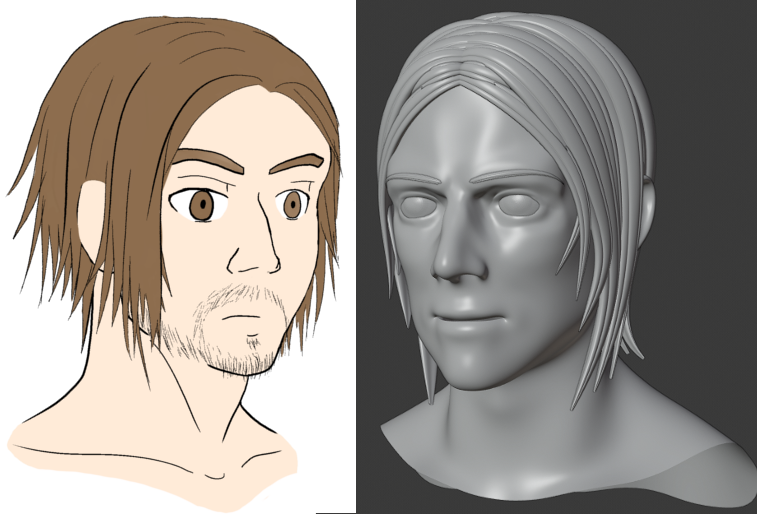
\includegraphics[width=.8\textwidth]{Figures/cap}
\decoRule
\caption[Capitano]{Modello 3D del volto del capt. Lawrence a confronto con il relativo concept.}
\label{fig:cap}
\end{figure}
\begin{figure}
\centering
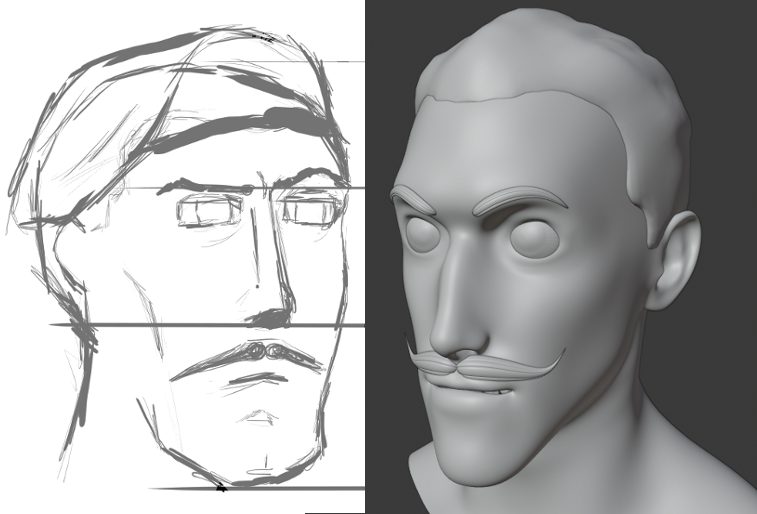
\includegraphics[width=.8\textwidth]{Figures/lt}
\decoRule
\caption[Tenente]{Modello 3D del volto del tenente a confronto con il relativo concept.}
\label{fig:lt}
\end{figure}
\begin{figure}
\centering
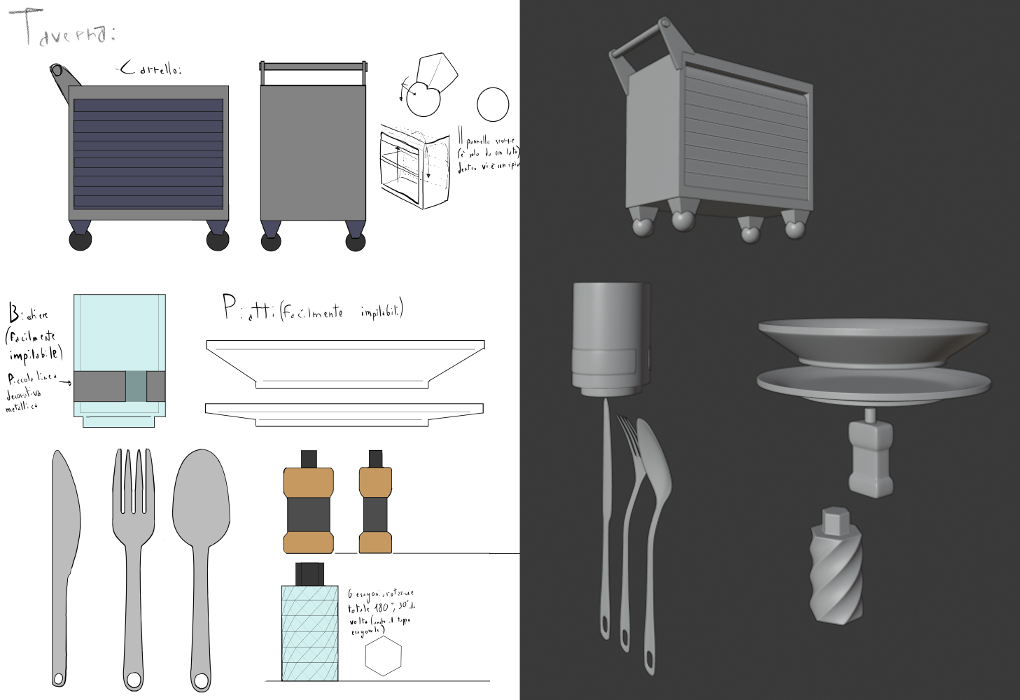
\includegraphics[width=.8\textwidth]{Figures/props}
\decoRule
\caption[Prop]{Alcuni modelli 3D dei prop a confronto con il relativo concept.}
\label{fig:prop}
\end{figure}

\newpage
\section{Texturing}

Il processo di texturing serve ad applicare un'immagine alla superficie di un oggetto, allo scopo di aggiungergli colore e dettagli di rilievo, detti appunto texture.  
Chiaramente i modelli rappresentati nelle figure non possono considerarsi completi senza l'aggiunta di colore.
Uno degli scopi delle texture è proprio questo, esse infatti permettono di mappare un'immagine sulla superficie della mesh.
Per fare ciò però, la mesh deve prima essere stesa su un piano. Questo è possibile farlo in maniera automatica, il problema è che spesso la topologia deve venire spezzata per poterla stendere su un piano.
In alternativa, per figure complesse, è consigliato farla manualmente, in modo da limitare i "tagli", che creerebbero discontinuità una volta applicata la texture.

Dopo aver eseguito questa procedura, è possibile creare una texture da associare a ciò che è stato ottenuto. Esistono diverse tecniche per fare ciò:
\begin{itemize}
    \item pittura manuale;
    \item generate proceduralmente.
    \item generata dalla geometria della mesh;
\end{itemize}
La prima, come suggerisce il nome, è la più artistica.
Si tratta fondamentalmente di disegnare sul modello.
Questa tecnica, seppure non sia affatto automatizzabile, è la più utilizzata, in quanto spesso non c'è altro modo di aggiungere dettagli irregolari. Essa è ad esempio stata usata per aggiungere il dettaglio ai capelli del capitano, per non dare l'idea che la sua chioma fosse un blocco unico, ma formato da tanti capelli.

Per i capelli di tutti gli altri personaggi, la texture è stata generata proceduralmente (vedi Figura \ref{fig:dialog}). Questo è stato possibile poiché, avendo questi altri, dei capelli lunghi, questi sono stati modellati con l'uso di curve in varie ciocche.
Dopodiché è stato possibile definire la texture in modo che fosse formata da tante linee che partissero da un estremo della curva all'altro.

Ad ogni modo le texture non sono usate solo per dare colore ad un oggetto. Esse sono utilizzate anche per aggiungere dettagli in rilievo.
Attraverso l'uso di particolari immagini, come mappe normali, che utilizzano i colori per rappresentare informazioni come la direzione della superficie, è possibile dare maggiore profondità ad un oggetto.
Questa tecnica è detta "baking", come era già stato menzionato in precedenza, permette di aggiungere dettagli ad un oggetto senza aumentarne il numero di vertici.
Il concetto che ne sta dietro è quello di pre-calcolare, una sola volta i dettagli, e poi applicarli al modello in bassa risoluzione.
In questo caso la texture viene generata direttamente dalla geometria della mesh.

\newpage
\section{Animazione e Rigging}

\begin{figure}
\centering
\begin{subfigure}{.33\textwidth}
  \centering
  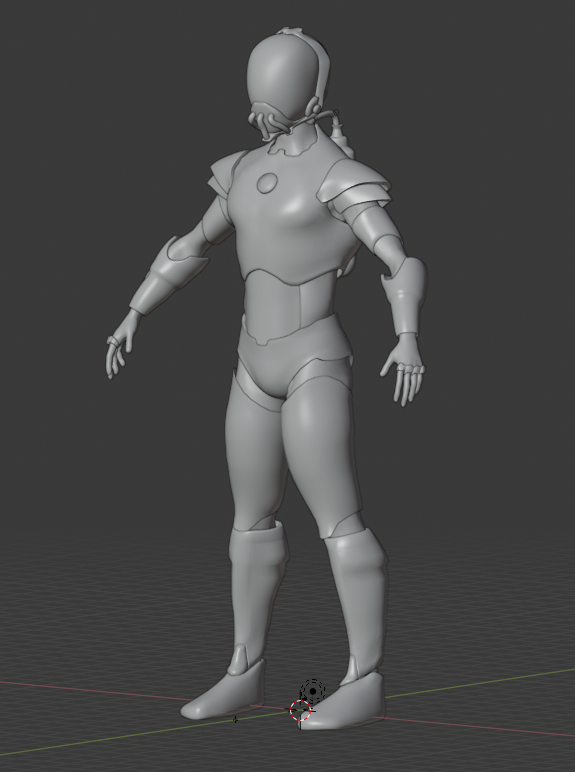
\includegraphics[width=\linewidth]{Figures/rig0}
  \caption{Modello senza controlli.\\}
  \vspace{13pt}
  \label{fig:rig0}
\end{subfigure}%
\begin{subfigure}{.33\textwidth}
  \centering
  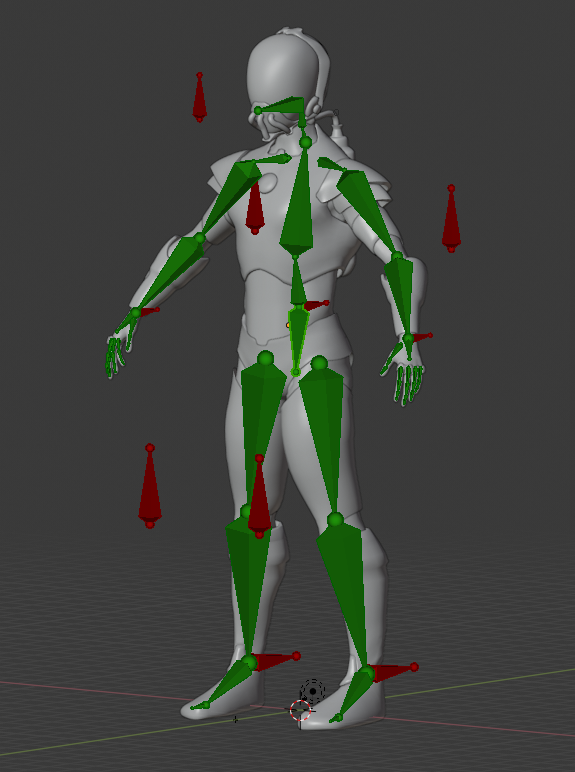
\includegraphics[width=\linewidth]{Figures/rig1}
  \caption{Armatura o meta-rig.}
  \bigskip
  \label{fig:rig1}
\end{subfigure}%
\begin{subfigure}{.33\textwidth}
  \centering
  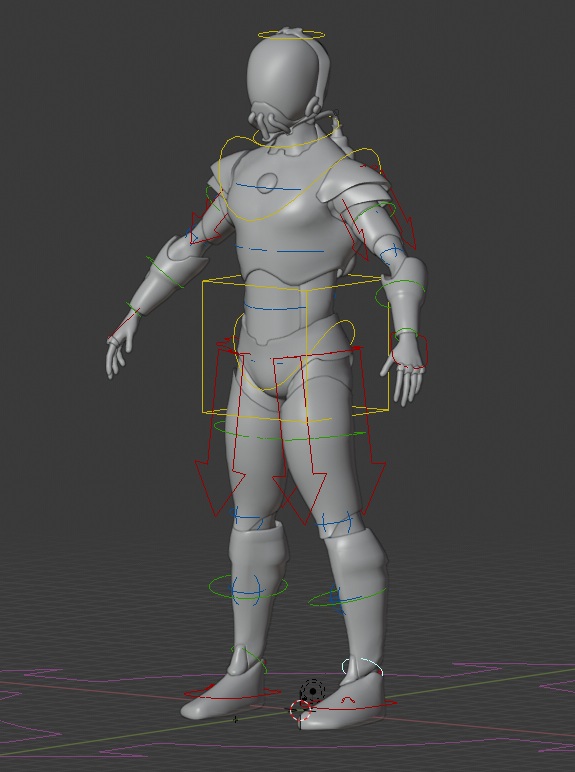
\includegraphics[width=\linewidth]{Figures/rig2}
  \caption{Rig avanzato con forme personalizzate.}
  \label{fig:rig2}
\end{subfigure}
\decoRule
\caption[Rig a confronto]{In figura è mostrato il modello di uno dei personaggi, con diversi tipi di controlli per l'animazione.}
\label{fig:rig}
\end{figure}

Rigging è un termine generale che si riferisce all'aggiunta di controlli ad un oggetto, tipicamente allo scopo di animarlo \parencite{blendDoc}.
Consiste nell'assegnare relazioni tra oggetti \parencite{BlendTut}.

Nel Capitolo \ref{Chapter4} è stato visto come progettare un rig orientato all'animazione che bisognerà eseguire.
Nella realizzazione di questi si è partiti definendo il meta-rig, aggiungendo tutte le ossa, dalla radice alle foglie, e associando ciascuna alla rispettiva porzione del modello, per permettere una deformazione soddisfacente di quest'ultimo.
Per generare il rig avanzato, è stato in parte usato rigify \cite{blendDoc}: una tecnologia che permette di automatizzare alcuni processi della realizzazione di un rig.
Purtroppo questa tecnologia è stata scoperta verso la fine del progetto e non è quindi stata utilizzata al massimo. 
Infatti i rig avanzati non sono quasi per nulla stati utilizzati, anche perché, essendo io e Uras già familiari nell'animare direttamente il meta-rig, si è preferito procedere direttamente alla realizzazione delle animazioni.
In Figura \ref{fig:rig} è possibile vedere il rig finito applicato ad un modello.
\begin{figure}
\centering
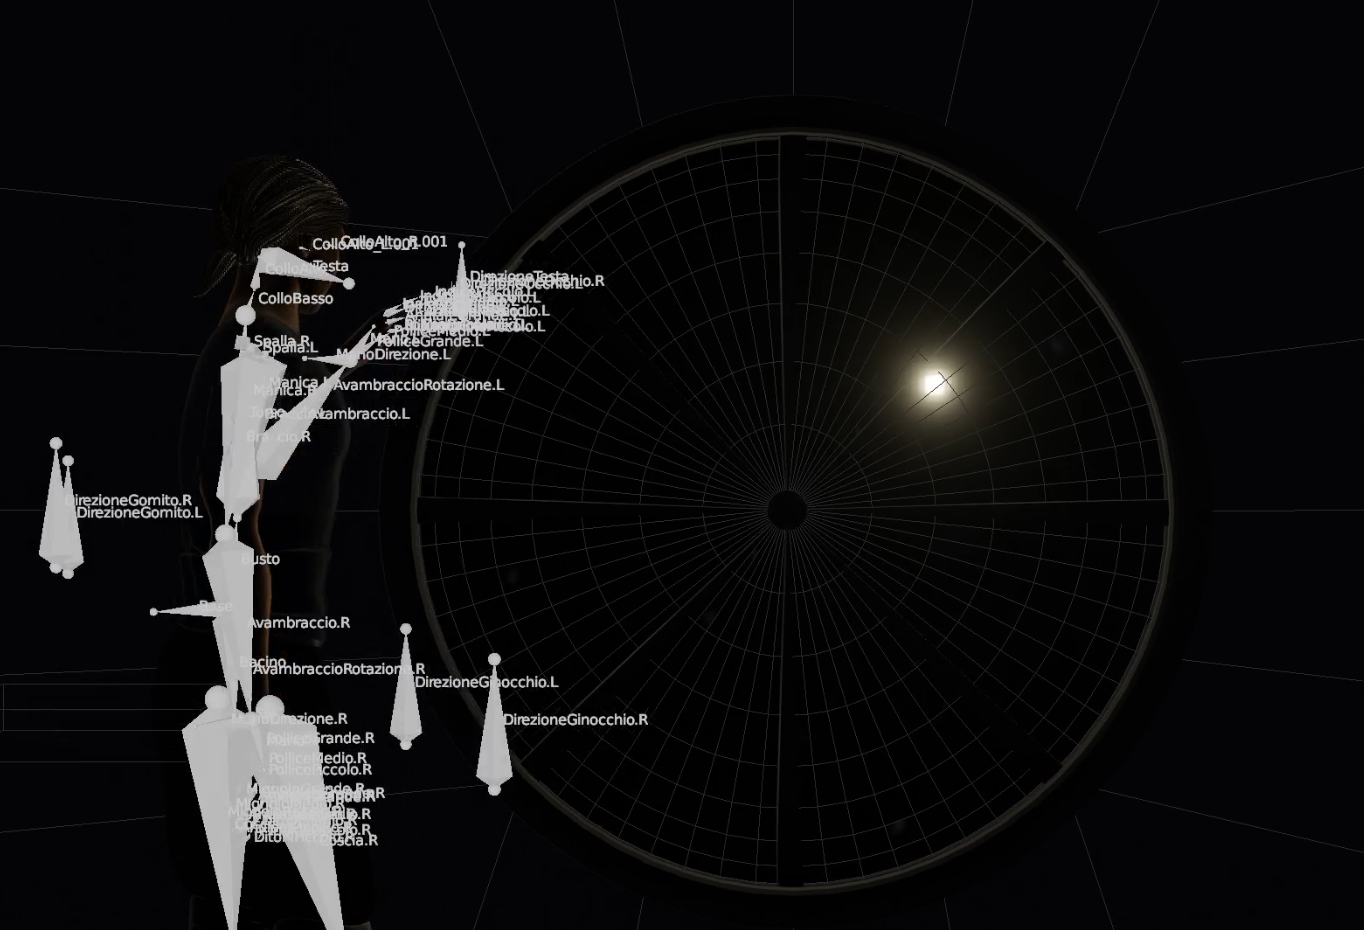
\includegraphics[width=\textwidth]{Figures/screen4}
\decoRule
\caption[Scena esempio 1]{In figura è rappresentata una delle prime scene, in cui il ragazzo si sveglia.}
\label{fig:eg1}
\end{figure}
\begin{figure}
\centering
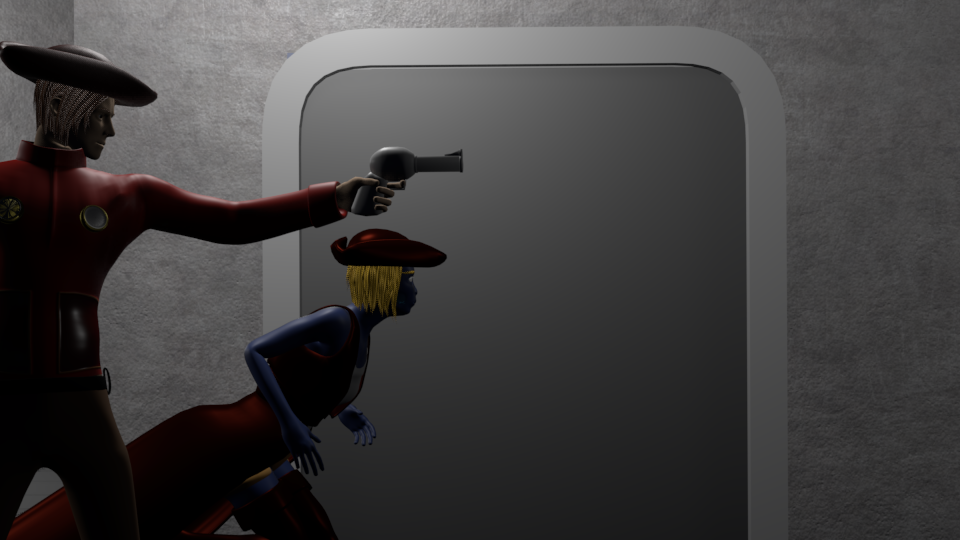
\includegraphics[width=\textwidth]{Figures/screen1}
\decoRule
\caption[Scena esempio 2]{In figura sono rappresentati capitano e capitana che si preparano ad uno scontro a fuoco.}
\label{fig:eg2}
\end{figure}
\begin{figure}
\centering
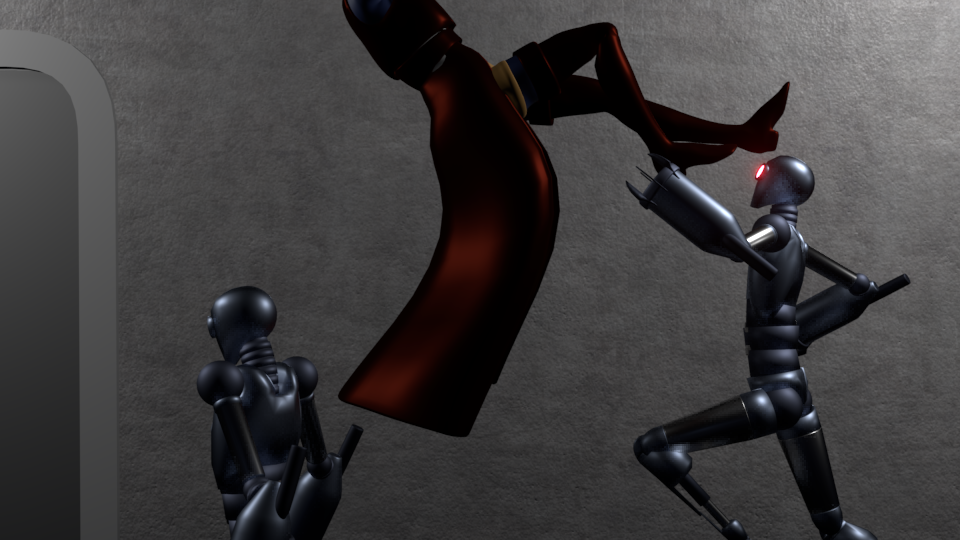
\includegraphics[width=\textwidth]{Figures/screen2}
\decoRule
\caption[Scena esempio 3]{In figura sono rappresentati due robot e la capitana, a mezz'aria, che sferra un calcio ad uno di essi.}
\label{fig:eg3}
\end{figure}

\subsection{Keyframe e metodi di animazione}
Ora che è possibile animare i modelli deformandoli, si può procedere con la realizzazione delle animazioni, precedentemente descritte al Capitolo \ref{Chapter4}.
Esistono principalmente due metodi di animazione \cite{Williams:2009:ASK:1823185}:
\begin{itemize}
    \item dall'inizio alla fine
    \item da posizione a posizione
\end{itemize}
Il primo è molto semplice: si parte dal primo frame, dove si posizionano all'interno della scena tutti i personaggi e la telecamera. Poi si passa al secondo animando ogni cosa, poi al terzo e così via. 
Questo metodo è molto utilizzato nell'animazione tradizionale, soprattutto nella realizzazione dei flip-book.
Ha il vantaggio di essere naturale: per arrivare in una determinata posizione devo spostarmi facendo un passo alla volta partendo dal primo punto in avanti.
Di conseguenza anche le animazione che ne risultano hanno un aspetto più naturale.
Questo metodo però rende difficile pianificare le azioni future per questo motivo non è ottimale.

\begin{figure}
\centering
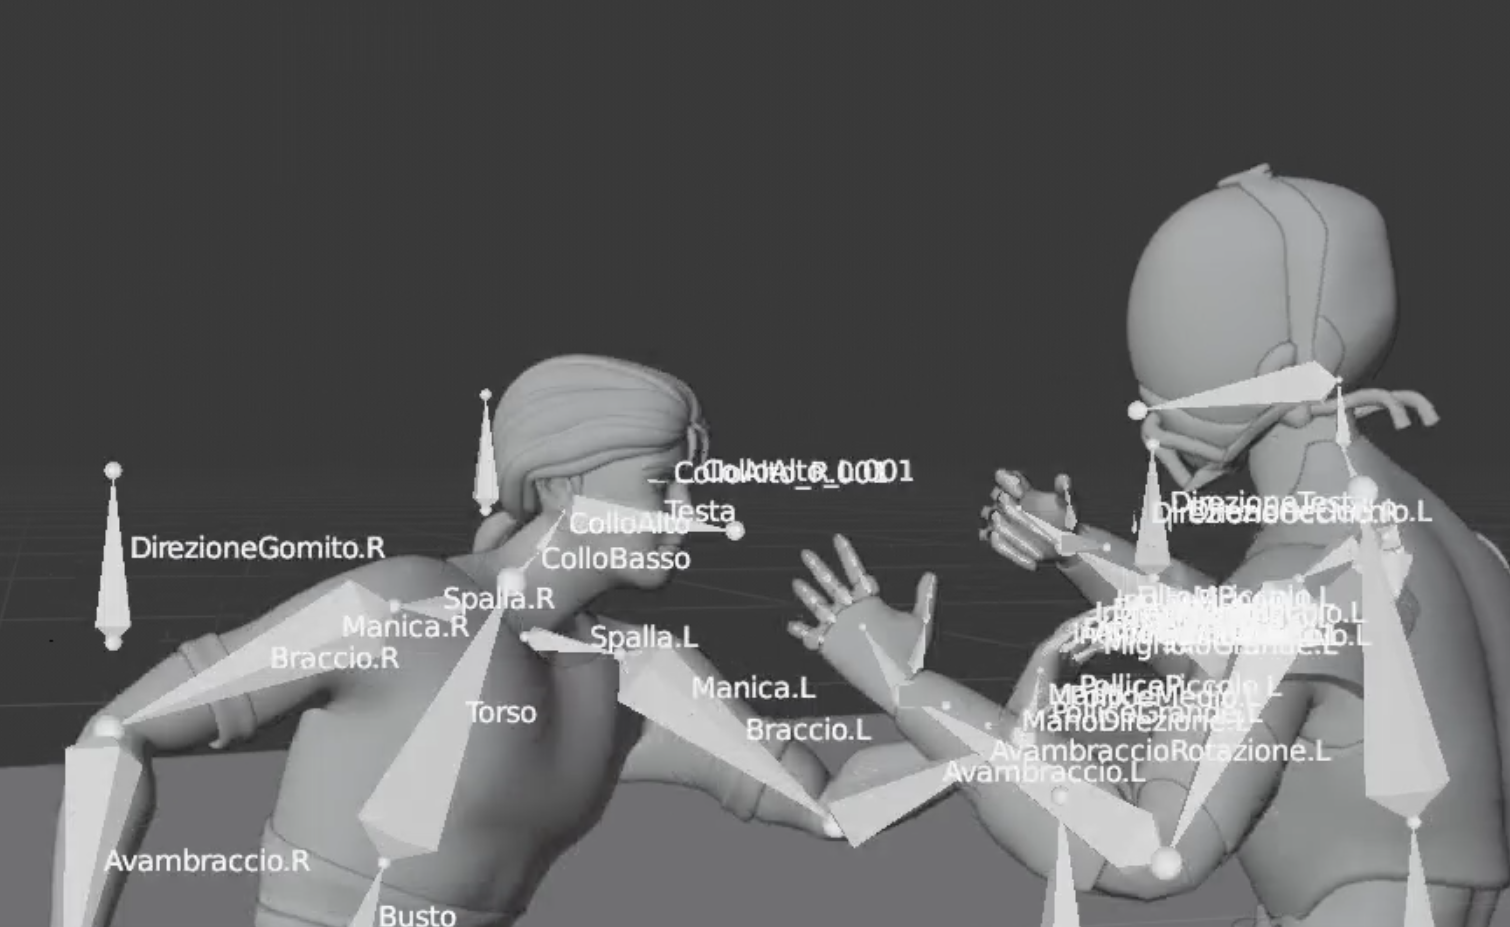
\includegraphics[width=\textwidth]{Figures/screen5}
\decoRule
\caption[Scena esempio 4]{In figura è rappresentato il ragazzo che spinge uno dei banditi spaziali.}
\label{fig:eg4}
\end{figure}
Al contrario, animare da posizione a posizione permette di pianificare un'intera scena definendo delle posizioni chiave.
Queste ultime, anche dette \emph{key-frame}, provengono direttamente dallo storyboard e definiscono cosa deve accadere in una scena.
Definite queste posizioni principali, distribuite nella sequenza dei frame della scena, si possono aggiungere i frame di intermezzo tra due posizioni.
Nell'animazione digitale questo metodo è il più efficiente in quanto i frame di intermezzo possono venire automaticamente calcolati come interpolazione delle due posizioni.
Il lato negativo è che le animazioni risultanti non sono molto naturali: spesso è necessario rendere un personaggio più veloce o più lento, per farlo arrivare in un ponto al tempo giusto e rispettare i piani preposti.

Per realizzare tutte le animazioni di questo cortometraggio è stato fatto ovviamente uso di quest'ultimo metodo.
Va aggiunto però che, per rendere le animazioni più naturali, dopo aver definito tutti i frame di intermezzo.
Questi ultimi sono stati modificati con un approccio dal primo verso l'ultimo.
In questo modo l'azione è più naturale, e spezza la linearità dell'interpolazione che, essendo calcolata dal computer, non mostra mai un movimento realistico fin da subito.
È quindi più giusto dire che nella realizzazione del trailer, è stato fatto uso di una combinazione delle due tecniche.
\begin{figure}
\centering
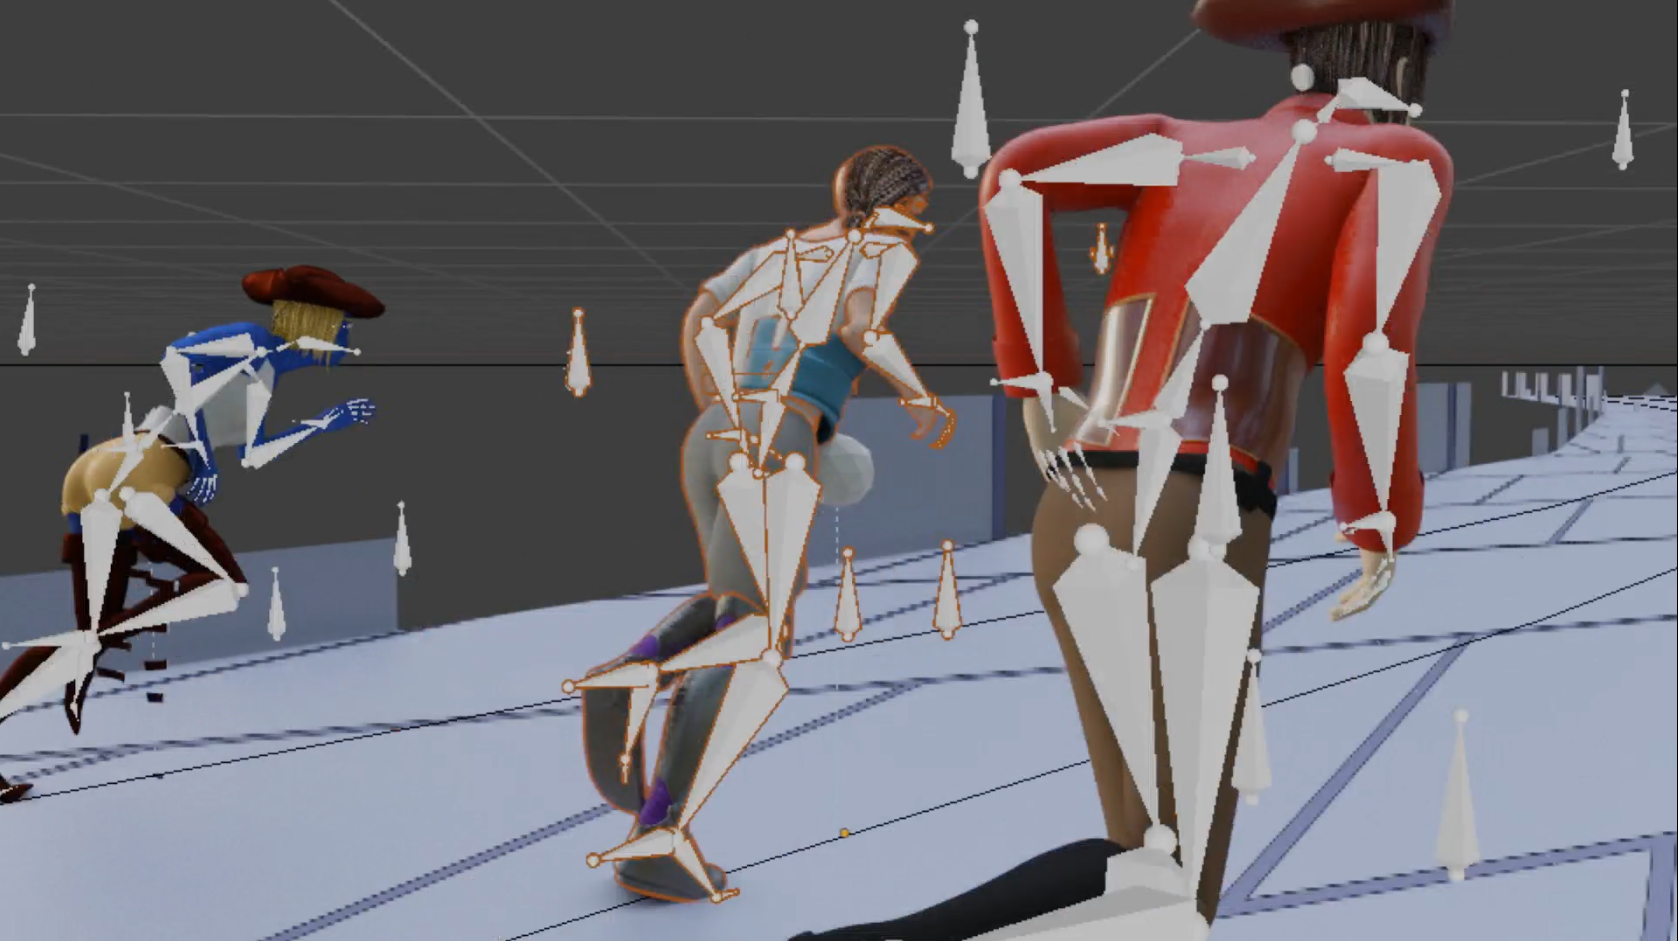
\includegraphics[width=\textwidth]{Figures/screen3}
\decoRule
\caption[Scena esempio 5]{In figura sono rappresentati Capitana, ragazzo e Capitano mentre corrono, per seminare i loro inseguitori.}
\label{fig:eg5}
\end{figure}

\subsection{Animazioni cicliche}
Inoltre, per le animazioni più comuni, esse sono state rese cicliche, per poterle iterare per la durata necessaria, e riutilizzarle in ogni scena necessaria.
In questo modo le animazioni sono state modularizzate, ovvero spezzate in più azioni ripetibili.
Alcune animazioni come la camminata, infatti, seguono dei pattern ben definiti, costituiti da varie fasi e,
grazie alla loro uniformità è possibile renderle cicliche in maniera tale da non dover rifare la stessa animazione più volte.

\begin{figure}
\centering
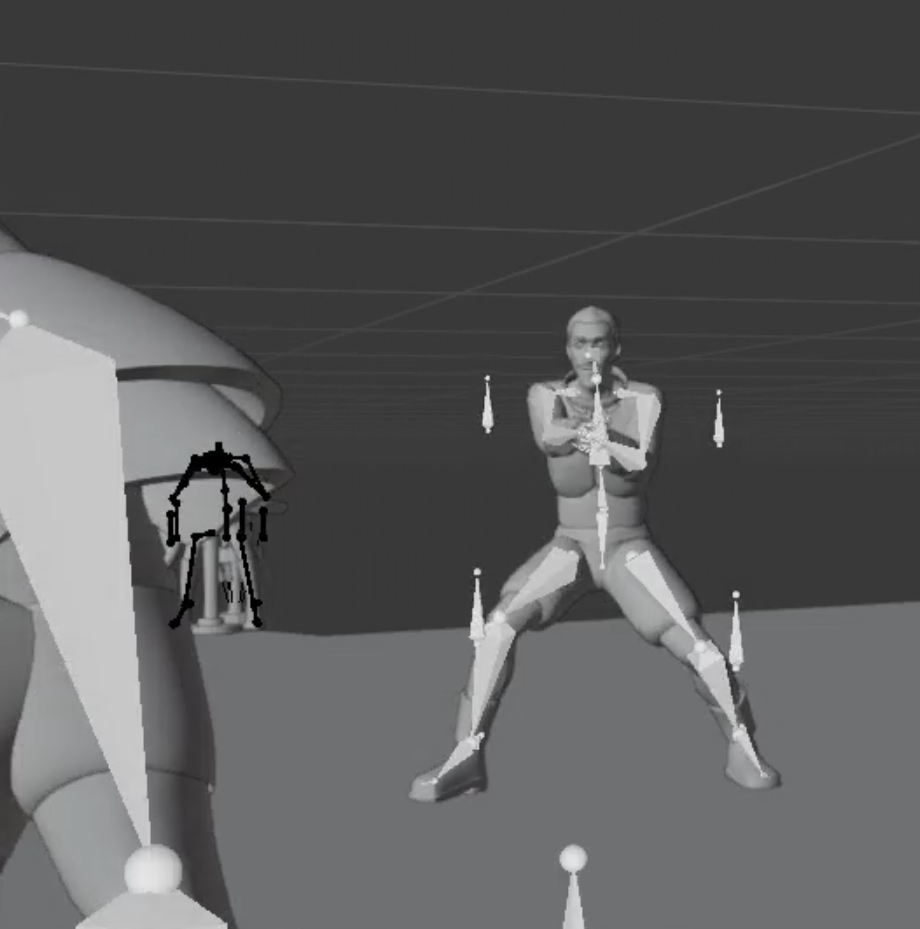
\includegraphics[width=\textwidth]{Figures/screen6}
\decoRule
\caption[Scena esempio 6]{In figura è rappresentato il tenente mentre spara ad uno dei banditi spaziali.}
\label{fig:eg6}
\end{figure}
Nel caso del ciclo della camminata queste fasi sono dette a supporto singolo e doppio supporto \cite{Parent:2012:CAA:2385444}.
Quest'ultima inizia con la posa di \emph{contatto}, in cui il secondo piede poggia a terra col tallone, e termina con la posizione di passaggio.
Viceversa la fase a singolo supporto inizia dalla posizione di passaggio e termina con la posizione di contatto.
Aggiungendo un solo frame di intermezzo per ogni fase, rispettivamente posa bassa (doppio contatto) e posa alta (contatto singolo), si ottiene un passo completo. Ripetendo il tutto per l'altra gamba l'animazione può considerarsi ultimata. I restanti frame verranno calcolati tramite interpolazione.

La corsa è molto simile alla camminata, ma differisce nella durata delle fasi e nel fatto che, a differenza della camminata, dove almeno un piede poggia sempre a terra, in questo entrambi i piedi non sono mai a contatto col suolo nello stesso momento.
Le due fasi sono quindi chiamate supporto singolo e volo, in cui nessun piede si trova a contatto col terreno.

Un volta ottenuta l'animazione ciclica, è possibile inserirla in ogni scena necessaria.
Nel caso di una camminata, è inoltre necessario spostare il modello mentre cammina.
Il modo migliore per farlo è quello di definire un percorso, che il modello dovrà seguire durante l'animazione.
Il percorso non è altro che una curva, solitamente NURBS o B-spline.
Il vantaggio di usare le curve in questo caso è che il percorso risultante avrà curve molto soffici.
Inoltre è possibile, attraverso i punti di controllo, modificare la curva a posteriori e, con essa, il modello si sposterà di conseguenza.

\begin{figure}
\centering
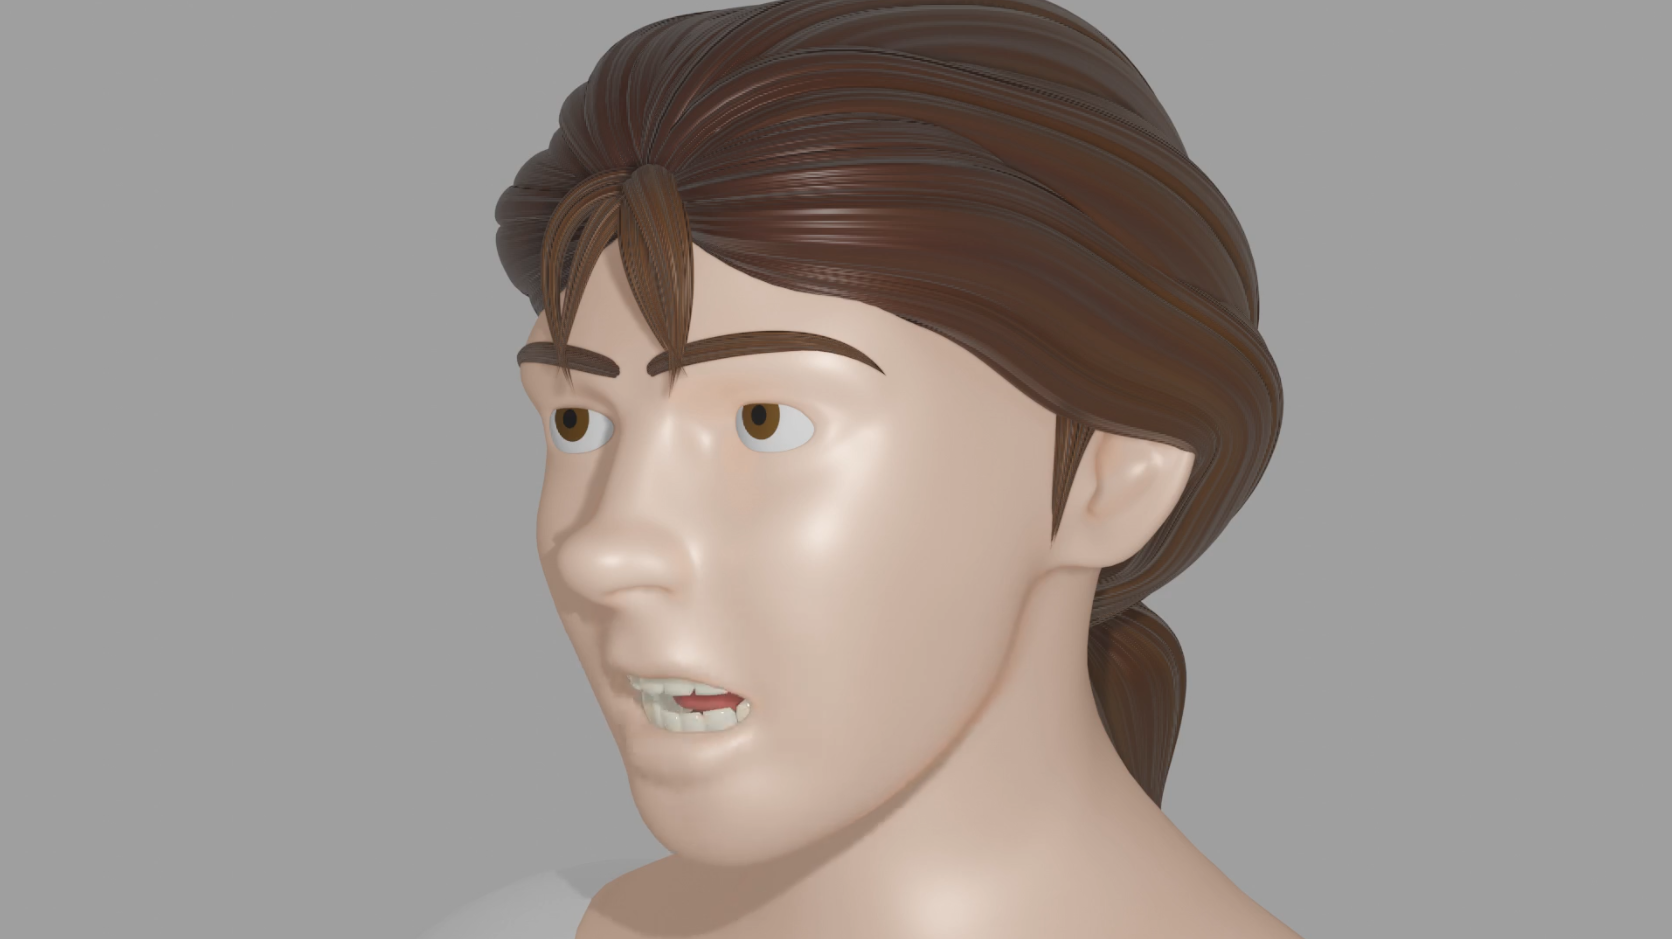
\includegraphics[width=\textwidth]{Figures/screen7}
\decoRule
\caption[Animazione dialoghi]{In figura è rappresentato il ragazzo mentre viene animato per un dialogo}
\label{fig:dialog}
\end{figure}
\subsection{Espressioni e Dialoghi}
Un altro aspetto importante delle animazioni, soprattutto in questo progetto, sono i dialoghi.
Nonostante si sia scelto di non doppiare i dialoghi dei personaggi, ma piuttosto tenere una traccia audio di sottofondo, per aggiungere drammaticità, è comunque stato necessario animare le facce dei personaggi per permettergli di parlare e esprimere sentimenti attraverso espressioni facciali.
Per fare ciò sono state utilizzate due tecnologie: \emph{shape-keys} \cite{blendDoc} e \emph{Rhubarb} \cite{blendRhubarb}.

Siccome la faccia è un concentrato di muscoli servirebbe un rig con centinaia di DOF.
Avere molte ossa per controllare ogni muscolo non è conveniente, poiché sarebbe difficile da animare.
Per semplificare il processo di animazione è conveniente parametrizzare ogni muscolo con una semplice variabile di range $0-1$ dove 0 indica il muscolo rilassato e 1 contratto.
Tuttavia a causa dell'elevato numero di muscoli presenti nella faccia sarebbe comunque difficile animare una singola espressione.
Un modo per ovviare a questo problema e quello di usare appunto delle shape-keys, conosciute anche come blend-shapes, dove ognuna rappresenta una posa della faccia (e.g. triste, felice, arrabbiato, sorpreso...), o meglio dividere ogni posa in aree della faccia e poi parametrizzarle e combinarle in modo che la loro somma sia uguale a 1.
Questo metodo è molto restrittivo rispetto al grado di controllo che ha l'animatore, poiché le espressioni rappresentabili dipendono dalle shape-keys definite precedentemente (e dalle loro combinazioni interpolanti).
Nonostante ciò rappresenta un buon compromesso tra semplicità d'uso e numero di espressioni rappresentabili.

Per quanto riguarda i dialoghi, Rhubarb Lyp Sync, permette di animare la bocca, e le aree limitrofe del viso, attraverso una traccia audio e scritta del dialogo da riprodurre.
Ciò è possibile perché a ogni fonema corrisponde un visema (i.e. espressione della faccia).
Per tanto, è stato sufficiente modellare un set limitato di espressioni e associarle ad il rispettivo fonema, registrare l'audio, e Rhubarb ha fatto il resto.
Come riportato da Parent \cite{Parent:2012:CAA:2385444}, esistono 42 diversi fonemi. Tuttavia molti di questi possono essere rappresentati dallo stesso visema, o da una interpolazione di questi.
Inoltre Williams afferma che non è necessario animare una frase in ogni sua singola sillaba, è sufficiente selezionare quelle più evidenti \cite{Williams:2009:ASK:1823185}. Questo ha permesso di ridurre il numero di shape-keys necessarie per i dialoghi a 9 che sono anche quelle utilizzate da Rhubarb.

\section{Illuminazione}

Quello dell'illuminazione è un passaggio fondamentale per poter renderizzare una scena. Infatti senza luci il risultato sarebbe ovviamente quello di una schermata nera.
Non solo, esistono diversi tipi di luce \cite{lightArt}, e da essi, oltre che dal loro posizionamento, l'aspetto di una scena può cambiare completamente.

Esistono fondamentalmente due categorie di settaggio di luci: per ambienti e per soggetti in primo piano.
Quest'ultimo è quello solitamente utilizzato dai fotografi nei loro studi fotografici: l'obiettivo è quello di creare una luce ad hoc, che risalti le forme del soggetto che si vuole rappresentare.
Questo è molto importante perché nella fotografia, così come nel rendering, si passa da una scena in tre dimensioni a una sua rappresentazione bidimensionale. 
È quindi facile perdere le informazioni di profondità, e le ombre servono proprio a questo. Solitamente per raggiungere questo scopo si utilizza un sistema a tre luci \cite{3Plight}.

L'illuminazione di un ambiente può spesso risultare più complessa. È importante indirizzare la luce per evidenziare cosa si vuole mostrare.
Il tutto è reso complesso dal fatto che ogni luce deve avere un contesto: aggiungere una luce che fluttua a mezz'aria non sarebbe realistico, bisogna che provenga da una fonte luminosa, come ad esempio una lampada.
Tutto comunque dipende dal contesto: non avrebbe senso aggiungere una lampada da tavolo in una scena all'esterno.

Indipendentemente dal tipo di scena che si vuole realizzare, il metodo in cui la luce viene calcolata per mostrare oggetti o oscurare l'ambiente circostante con ombre è sempre lo stesso, e dipende dal motore di renderizzazione.

\section{Renderizzazione}

Il processo di renderizzazione è ciò che permette di proiettare la scena tridimensionale in un’immagine in una finestra contenuta nello schermo bidimensionale \cite{renderingPipelineDLazzaro}.
Per fare ciò, è necessario definire una camera virtuale, attraverso un punto nello spazio tridimensionale che ne definisce la posizione, un vettore che indica la direzione in cui essa è orientata, un angolo che definisce il campo visivo ed infine la profondità oltre la quale non è necessario renderizzare.

Attraverso una serie di trasformazioni, ogni oggetto presente nella scena viene proiettato nel sistema di riferimento della telecamera.
Esiste comunque più di un modo per calcolare queste trasformazioni, due di questi sono rasterizzazione e ray-tracing.

Nel primo caso il calcolo è incentrato sugli oggetti presenti nella scena. Per ognuno di essi viene tracciato un raggio che parte da ogni vertice verso la telecamera.
Collegando i punti sulla griglia di visualizzazione, è possibile capire quale area dello schermo l'oggetto ricopre.
Dopodiché attraverso un buffer di profondità viene calcolato quali oggetti sono più vicino alla camera e quindi coprono gli oggetti più lontani.
Questo è un processo relativamente veloce perché il numero di raggi è limitato al numero di vertici presenti nella scena.
Di fatti, questo è il metodo che fino a qualche anno fa veniva usato in tutti i videogiochi per permettere una renderizzazione in tempo reale.
Questo spiega anche perché nei videogiochi ci sia la tendenza a tenere un numero di vertici molto più basso rispetto ad un film realizzato con la computer grafica.
Tuttavia, questo metodo presenta lo svantaggio di non riuscire a calcolare le luci in maniera realistica.

Il secondo metodo invece è incentrato sulla vista: dalla telecamera viene proiettato un raggio che interseca la griglia di visualizzazione per ogni pixel dell'immagine risultante.
Questi raggi, detti primari, continuano in linea retta finché non trovano un oggetto.
Dal punto di incidenza con l'oggetto, dipendentemente dalle proprietà fisiche di quest'ultimo, partono altri raggi, alcuni sono quelli secondari, che si dirigono direttamente verso le sorgenti luminose, per capire se l'oggetto è illuminato direttamente, oppure esiste un altro oggetto che proietta un ombra.
I restanti sono raggi di riflessione/rifrazione e permettono di calcolare la luce ambientale o indiretta che non era possibile calcolare nella rasterizzazione.
Per via dell'alto numero di computazioni necessarie, questo è un metodo molto più lento rispetto al primo, ma permette di raggiungere risultati molto più fotorealistici.

Recentemente comunque quest'ultimo metodo, è stato velocizzato a tal punto da poter essere implementato nei videogiochi, con una renderizazione in tempo reale.
Il primo invece è stato sviluppato a tal punto da ottenere immagini fotorealistiche, quasi quanto il secondo.
Blender propone due motori di renderizzazione, ognuno implementante uno di questi due metodi, rispettivamente Eevee e Cycles.

Nella realizzazione di questo cortometraggio è stato scelto di utilizzare Eevee come motore di renderizzazione. 
Il motivo di questa scelta deriva dal fatto che ciò ci ha permesso di accorciare notevolmente i tempi di rendering, al costo di un risultato meno realistico, che comunque non era uno dei requisiti.